
\graphicspath{{./fig5/}}

%
\section{RICC}
\label{sec:ricc}
本節では,理化学研究所のRICCシステム\footnote{http://accc.riken.go.jp/ricc.html}環境でのコンパイルについて示す.

RICCシステムでは幾種類かのコンパイラとMPIライブラリが利用可能なので,各ライブラリに合わせてコンパイルを行う.
ここでは,OpenMPIと富士通MPIについて示す.

\begin{itemize}
\item OpenMPI\\
V-Sphereのコンパイル前に,以下の修正を行う.
\begin{enumerate}
\item \verb|libmpi_cxx.so.0|のバスの設定\\
以下のコマンドを実行して,\verb|libmpi_cxx.so.0|のパスの指定を行う\footnote{後述のインストールシェルを利用する場合には,シェルに書き込んであるが,~/.bashrcに書いておくと良い.sphPrjToolの使用時にも必要.}.
{ \small
\begin{program}
$ export LD_LIBRARY_PATH=/usr/local/openmpi/intel/lib:$LD_LIBRARY_PATH
\end{program}}
\vspace{2mm}

\item \verb|CLTK_TARGET_MACHINE|の指定\\
homeディレクトリで\verb|.cltkrc|というファイルを作成し,以下の情報を記述する.
{ \small
\begin{program}
CLTK_TARGET_MACHINE = pc
\end{program}}
\vspace{2mm}

\item コンパイル\\
後述のインストールシェルを用いてインストールする.シェルの引数にはインストール先のディレクトリをフルパスで指定する.RICCではユーザは,自分の管理ディレクトリにインストールすること.
{ \small
\begin{program}
$ configure_ic_ompi.sh INSTALL_DIR
$ make
$ make install
\end{program}}
\vspace{2mm}

富士通コンパイラを利用する場合には,\verb|include/SklTiming.h|ファイルに,以下のインクルード文を追加する\footnote{V-Sphereで対応予定.}.
{ \small
\begin{program}
#include <stdio.h>
\end{program}}
\vspace{2mm}
\end{enumerate}

%
\item Fujitsu MPI\\
\begin{enumerate}
\item \verb|CLTK_TARGET_MACHINE|の指定\\
homeディレクトリで\verb|.cltkrc|というファイルを作成し,以下の情報を記述する.
{ \small
\begin{program}
CLTK_TARGET_MACHINE = pc
\end{program}}
\vspace{2mm}

\item \verb|_USE_SKL_FSEEK|の定義\\
\verb|include/endianUtil.h|ファイルに以下の記述を追加する\footnote{富士通MPIを使用時にfseekのSEEK\_SETやSEEK\_CURが使用できないため.今後対応予定.}.
{ \small
\begin{program}
#define _USE_SKL_FSEEK
\end{program}}
\vspace{2mm}

\item \verb|-lmpi|の指定の削除\\
\verb|src/utility/sphDataGather/Makefile|内に記述されている\verb|-lmpi|の指定を以下のようにコメントアウトする\footnote{富士通MPIを使用時にsphDataGatherの Makefile内でlmpiについてのエラーが出るため.今後対応予定.}.
{ \small
\begin{program}
MPICH_LIBS = #-lmpi
dataGather_LDADD = -lsphcfg #-lmpi 
sphDataGather_LDADD = -lsphcfg #-lmpi
\end{program}}
\vspace{2mm}

\item コンパイル\\
{ \small
\begin{program}
$ ./configure または インストールシェル
$ make
$ make install
\end{program}}
\end{enumerate}

%
\item インストールシェル\\
コンパイラとMPIライブラリーの組み合わせにより,次のインストールシェルが利用できる.
これらのシェルの引数をディレクトリ名としてV-Sphereをインストールする.
どの場合にも,倍精度計算の場合には\verb|--with-real=double|を追加する.
\begin{indentation}{3zw}{0zw}
\small
\begin{program}
------------------------------------
Intelコンパイラ+OpenMPI  configure_ic_ompi.sh
------------------------------------
#! /bin/sh
export LD_LIBRARY_PATH=/usr/local/openmpi/intel/lib:$LD_LIBRARY_PATH
 ./configure --prefix=$1 \
             --with-comp=INTEL \
             --with-ompi=/opt/FJSVcltk/bin \
             FC="mpif77 -intel -openmpi" \
             FCFLAGS=-O3 \
             F90="mpif90 -intel -openmpi" \
             F90FLAGS=-O3 \
             CC= "mpicc -intel -openmpi" \
             CFLAGS= -middle \
             CXX= "mpic++ -intel -openmpi" \
             CXXFLAGS= -O3 \
             LDFLAGS= "-L/opt/intel/Compiler/11.1/046/lib/intel64" \

------------------------------------
富士通コンパイラ+富士通MPI  configure_fc_fmpi.sh
------------------------------------
#! /bin/sh
export LD_LIBRARY_PATH=/usr/local/openmpi/intel/lib:$LD_LIBRARY_PATH
 ./configure --prefix=$1 \
             --with-comp=FJ \
             --with-ompi=/opt/FJSVcltk/bin \
             FC="mpif77 -fj -fjmpi" \
             FCFLAGS=-O3 \
             F90="mpif90 -fj -fjmpi" \
             F90FLAGS=-O3 \
             CC= "mpicc -fj -fjmpi" \
             CFLAGS= -O3 \
             CXX= "mpic++ -fj -fjmpi" \
             CXXFLAGS= -O3 \
             LDFLAGS= "-L/opt/intel/Compiler/11.1/046/lib/intel64" \

------------------------------------
Intelコンパイラ+富士通MPI  configure_ic_fmpi.sh
------------------------------------
#! /bin/sh
export LD_LIBRARY_PATH=/usr/local/openmpi/intel/lib:$LD_LIBRARY_PATH
 ./configure --prefix=$1 \
             --with-comp=INTEL \
             --with-ompi=/opt/FJSVcltk/bin \
             FC="mpif77 -intel -fjmpi" \
             FCFLAGS=-O3 \
             F90="mpif90 -intel -fjmpi" \
             F90FLAGS=-O3 \
             CC= "mpicc -intel -fjmpi" \
             CFLAGS= -middle \
             CXX= "mpic++ -intel -fjmpi" \
             CXXFLAGS= -O3 \
             LDFLAGS= "-L/opt/intel/Compiler/11.1/046/lib/intel64" \
\end{program}
\end{indentation}


\end{itemize}


%
\hypertarget{tgt:BGL}{\section{IBM BlueGene/L}}

本節では,IBM BlueGene/L\index{BlueGene}でのコンパイルについて説明する.コンパイル環境は,IBM XLFortran, XLC++コンパイラ,クロスコンパイルである.

\subsection{libxml2(2.6.30)}
\begin{enumerate}
\item configure
--prefixだけ変更すること.(libxml2インストールディレクトリ)
{\small
\begin{program}
$ user@quadro:~/XML2/libxml2-2.6.30> ./configure --prefix=/gfs1/user/XML2 CC=blrts_xlc  
CXX=blrts_xlC F77=blrts_xlf CFLAGS="-DLIBXML2_STATIC -O3 -qarch=440d -qtune=440 
-I/bgl/BlueLight/ppcfloor/bglsys/include" CXXFLAGS="-O3 -qarch=440d -qtune=440 
-I/bgl/BlueLight/ppcfloor/bglsys/include" FFLAGS="-O3 -qarch=440d -qtune=440 
-I/bgl/BlueLight/ppcfloor/bglsys/include" LDFLAGS="-L/bgl/BlueLight/ppcfloor/bglsys/lib 
-lmpich.rts -lmsglayer.rts -lrts.rts -ldevices.rts" --enable-shared=no --without-threads 
--without-python --without-ftp --without-http --without-readline --disable-ipv6
\end{program}
}

\item make
testapi,runtest(サンプルソース?)でリンクエラーが出る.Makefileのリンクをしている行をコメントにしてmakeする.
{\small
\begin{program}
L.702
# $(LINK) $(runtest_LDFLAGS) $(runtest_OBJECTS) $(runtest_LDADD) $(LIBS)

L.741
# $(LINK) $(testapi_LDFLAGS) $(testapi_OBJECTS) $(testapi_LDADD) $(LIBS)
\end{program}
}
\item make install\\
{\small
\begin{program}
$ make install
\end{program}
}
\end{enumerate}

\subsection{V-sphere}
Makefile.specを使用してmakeを実行する.以下の例では,V-Sphere version 1.4.1を用いた記述になっている.

\begin{enumerate}

\item Config.specの編集\\
変更箇所は以下のとおりである.\footnote{INSTALLDIR, XML2FLAGS, XML2LIBSは,ユーザ毎の設定になる.INSTALLDIRは,sphereライブラリをインストールするディレクトリを指定すること.XML2FLAGS, XML2LIBSは,「/gfs1/user/XML2」を指定したlibxml2インストールディレクトリ(--prefix)に置き換えること.}
{\small
\begin{program}
INSTALLDIR      = /gfs1/user/sphere/Vsphere_1_4_1_lib
CXXCOMPTYPE     = IBM
CXXDIR          = /usr
CXXCOMP         = blrts_xlC
CXXOPT          = -qarch=440 -qtune=440 -O3 -D_NON_P4_DEVICE_

CCOMPTYPE       = IBM
CCDIR           = /usr
CCOMP           = blrts_xlc
COPT            = $(CXXOPT)

FCOMPTYPE       = IBM
FCDIR           = /usr
FCOMP           = blrts_xlf
FCOPT           = $(CXXOPT)

F90COMPTYPE     = IBM
F90DIR          = /usr
F90COMP         = blrts_xlf90
F90OPT          = $(CXXOPT)

MPICH_DIR       = /bgl/BlueLight/ppcfloor/bglsys
XML2FLAGS       = -I/gfs1/user/XML2/include/libxml2
XML2LIBS        = -L/gfs1/user/XML2/lib -lxml2
RANLIB          = echo
\end{program}
}

\item Makefile.specの編集
変更箇所は以下のとおり.
{\small
\begin{program}
MPI_LIBS = -lmpich
     ↓
MPI_LIBS = -lmpich.rts -lmsglayer.rts -lrts.rts -ldevices.rts
\end{program}
}

\item make、installの実行
{\small
\begin{program}
$ make -f Makefile.spec
$ make -f Makefile.spec install
\end{program}
}

\end{enumerate}

%
\section{AMD Opteron}

本節では,AMD Opteron\index{AMD Opteron}上でのsphereコンパイルについて述べる.コンパイラをPGIコンパイラとしている.

\begin{enumerate}
\item configure
{\small
\begin{program}
$ ./configure --prefix=/gfs1/user/sphere/Vsphere_1_4_1_lib --with-mpich=/usr/local/mpich 
FC=pgf77 FCFLAGS=-O3 F90=pgf90 F90FLAGS=-O3 CXX=pgCC CXXFLAGS="-O3 -D_NON_P4_DEVICE_"
\end{program}
}

\item Vcarソース修正
SklVcarManifest.Cで\_ATOLのエラーが出るので,ソースの先頭付近に以下の行を追加する.
\small \verb|#define _ATOL atol|

\item make
{\small
\begin{program}
$ make
$ make install
\end{program}
}

\end{enumerate}


%
\section{QUEST}
\label{sec:install_quest}
本節では,理化学研究所のQuestシステム\footnote{Questシステムの詳細については,VPN経由で,http://quest.q.riken.jp}(PFU製RG1000$\times$64台, 1024node, 1CPU/node, 2cores/CPU, 2GB/node, GE)環境でのコンパイルについて示す.
Questシステムでは幾種類かのMPIライブラリが利用可能なので,各ライブラリに合わせてコンパイルを行う.下記に,インストールシェルのサンプルを示す.

倍精度のモジュールを作成する場合には,\verb|--with-real=double|を追加すること.

\begin{indentation}{3zw}{0zw}
\small
\begin{program}
------------------------------------
configure_mpich.sh \\ Intel Compiler + mpich
------------------------------------
#! /bin/sh
#
# at .bashrc
#
# QUEST_COMPILER_TYPE=intel
# QUEST_MPI_TYPE=mpich
# [ -f /opt/FJSVcltk/etc/questrc.sh ] && source /opt/FJSVcltk/etc/questrc.sh
#

 ./configure --prefix=$1 \
             --with-comp=INTEL \
             --with-mpich=/usr/local/mpich/intel \
             --enable-nop4dev \
             FC=/opt/intel/Compiler/11.0/081/bin/intel64/ifort \
             FCFLAGS=-O3 \
             F90=/opt/intel/Compiler/11.0/081/bin/intel64/ifort \
             F90FLAGS=-O3 \
             CC=/opt/intel/Compiler/11.0/081/bin/intel64/icc \
             CFLAGS=-O3 \
             CXX=/opt/intel/Compiler/11.0/081/bin/intel64/icpc \
             CXXFLAGS=-O3 \
             LDFLAGS=-L/opt/intel/Compiler/11.0/081/lib/intel64 \

------------------------------------
configure_ompi.sh \\ Intel Compiler + openmpi
------------------------------------
#! /bin/sh
#
# at .bashrc
#
# QUEST_COMPILER_TYPE=intel
# QUEST_MPI_TYPE=openmpi
# [ -f /opt/FJSVcltk/etc/questrc.sh ] && source /opt/FJSVcltk/etc/questrc.sh
#
 ./configure --prefix=$1 \
             --with-comp=INTEL \
             --with-ompi=/usr/local/openmpi/intel \
             --enable-nop4dev \
             FC=/opt/intel/Compiler/11.0/081/bin/intel64/ifort \
             FCFLAGS=-O3 \
             F90=/opt/intel/Compiler/11.0/081/bin/intel64/ifort \
             F90FLAGS=-O3 \
             CC=/opt/intel/Compiler/11.0/081/bin/intel64/icc \
             CFLAGS=-O3 \
             CXX=/opt/intel/Compiler/11.0/081/bin/intel64/icpc \
             CXXFLAGS=-O3 \
             LDFLAGS=-L/opt/intel/Compiler/11.0/081/lib/intel64 \

------------------------------------
configure_ompi_dbl.sh \\ Intel Compiler + openmpi, double precision
------------------------------------
#! /bin/sh
#
# at .bashrc
#
# QUEST_COMPILER_TYPE=intel
# QUEST_MPI_TYPE=openmpi
# [ -f /opt/FJSVcltk/etc/questrc.sh ] && source /opt/FJSVcltk/etc/questrc.sh
#
 ./configure --prefix=$1 \
             --with-comp=INTEL \
             --with-ompi=/usr/local/openmpi/intel \
             --enable-nop4dev \
             --with-real=double \
             FC=/opt/intel/Compiler/11.0/081/bin/intel64/ifort \
             FCFLAGS=-O3 \
             F90=/opt/intel/Compiler/11.0/081/bin/intel64/ifort \
             F90FLAGS=-O3 \
             CC=/opt/intel/Compiler/11.0/081/bin/intel64/icc \
             CFLAGS=-O3 \
             CXX=/opt/intel/Compiler/11.0/081/bin/intel64/icpc \
             CXXFLAGS=-O3 \
             LDFLAGS=-L/opt/intel/Compiler/11.0/081/lib/intel64 \
             
------------------------------------
configure_impi.sh \\ Intel Compiler + Intelmpi
------------------------------------
#! /bin/sh
#
# at .bashrc
#
# QUEST_COMPILER_TYPE=intel
# QUEST_MPI_TYPE=intelmpi
# [ -f /opt/FJSVcltk/etc/questrc.sh ] && source /opt/FJSVcltk/etc/questrc.sh
#
 ./configure --prefix=$1 \
             --with-comp=INTEL \
             --with-ompi=/opt/intel/impi/3.2 \
             --enable-nop4dev \
             FC=/opt/intel/Compiler/11.0/081/bin/intel64/ifort \
             FCFLAGS=-O3 \
             F90=/opt/intel/Compiler/11.0/081/bin/intel64/ifort \
             F90FLAGS=-O3 \
             CC=/opt/intel/Compiler/11.0/081/bin/intel64/icc \
             CFLAGS=-O3 \
             CXX=/opt/intel/Compiler/11.0/081/bin/intel64/icpc \
             CXXFLAGS=-O3 \
             LDFLAGS=-L/opt/intel/Compiler/11.0/081/lib/intel64 \    
\end{program}
\end{indentation}


%
\section{Windows}
以下の環境でV-Sphere.exeモジュールの作成を実施した.

\begin{itemize}
\item WindowsXP sp3 32bit
\item Microsoft Visual Studio 2008
\item Intel Compiler 10.1.021
\item MPICH2  ver 1.0.7
\item libxml2, zlib, iconvのインストールパス\\
C:{\yen}Program Files{\yen}ext\_libs{\yen}libxml2\\
C:{\yen}Program Files{\yen}ext\_libs{\yen}zlib\\
C:{\yen}Program Files{\yen}ext\_libs{\yen}iconv\\
\end{itemize}

%
\subsection{V-Sphereのインストール}
V-SphereのWindowsインストーラの\lq\lq setup\_sphere.msi\rq\rq を起動してV-Sphereをインストールする.
デフォルト設定では,以下のフォルダ,ファイルがインストールされる.

\begin{program}
C:\Program Files\sphere
├─bin
│      dataGather.exe
│      sphCfgTool.exe
│      sphCfgTool.exe.config
│      sphDataGather.exe
│      sphMbxTool.exe
│      sphPrjTool.exe
│      
├─config
│      sph-cfg.xml
│      
├─doc
│      
├─html
│      
├─include
│  │  DebugLog.h
│  │  endianUtil.h
│  │  Skl.h
│  │  SklBase.h
│  │  SklDefine.h
│  │  SklGloval.h
│  │  sklparaf.h
│  │  SklReservWord.h
│  │  SklSolverBase.h
│  │  SklSolvFactoryBase.h
│  │  SklTiming.h
│  │  SklUtil.h
│  │  SklVersion.h
│  │  SklXMLType.h
│  │  sph_win32_util.h
│  │  utilPath.h
│  │  vfvPathUtil.h
│  │  
│  ├─base
│  ├─config
│  ├─coord
│  ├─dataclass
│  ├─fileio
│  ├─ftt
│  ├─linearsolver
│  ├─parallel
│  └─vcar
│          
└─lib
        libsphapp.lib
        libsphbase.lib
        libsphcfg.lib
        libsphcrd.lib
        libsphdc.lib
        libsphfio.lib
        libsphftt.lib
        libsphls.lib
        libsphparadmy.lib
        libsphparampi.lib
        libsphvcar.lib

\end{program}

%
\subsection{環境設定}
プロジェクトツールによるソルバのproject\_local\_settings,Makefile.winを作成する為に,\lq\lq sphCfgTool.exe\rq\rq を起動する\textbf{図\ref{fig:sphCfgTool setting}}\footnote{C:{\yen}Program Files{\yen}sphere{\yen}bin{\yen}sphCfgTool.exe}.

\begin{figure}[htbp]
\begin{center}
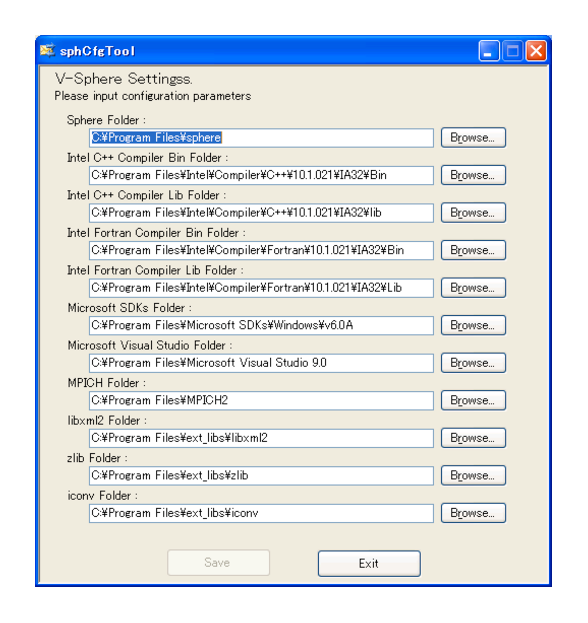
\includegraphics[width=8cm,clip]{sphCfgTool.eps}
\end{center}
\caption{sphCfgToolの設定画面}
\label{fig:sphCfgTool setting}
\end{figure}

\lq\lq sphCfgTool.exe\rq\rq は、インストール中にも起動される.
インストール後は,直接\lq\lq sphCfgTool.exe\rq\rq を起動するか、プログラムメニュー「Sphere」-「sphCfgTool」から起動.
sphCfgToolの画面で,パスの設定が異なっていると赤字\textbf{図\ref{fig:sphCfgTool error}}で\lq\lq Invalid Folder\rq\rq が表示される.
すべてパス設定が行われていることを確認する.

\begin{figure}[htbp]
\begin{center}
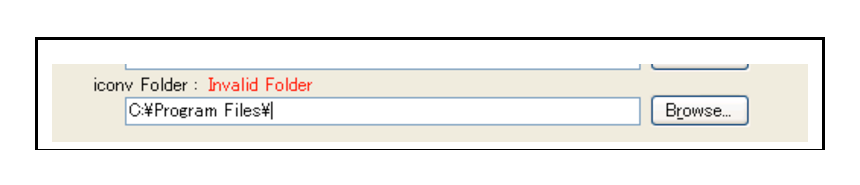
\includegraphics[width=10cm,clip]{error.eps}
\end{center}
\caption{sphCfgToolのパスの設定エラー}
\label{fig:sphCfgTool error}
\end{figure}




